% paper/main.tex
% v2 — Fable, 2026-08-26 — post-audit rewrite (bd tns-2ze); statuses as of
% claims/CLAIMS.md @ the corpus-r4 fixed point (theory/verdicts/corpus-r4.md).
% ============================================================================
% Prose register target: refs/arxiv-1305.2176/paper_final.tex (PRL 111, 080401).
% Prose rules: docs/prose-guide.md (binding).
% Every claim-bearing sentence traces to a claims/CLAIMS.md row; the map is
% paper/v2-claim-audit.md. Conjectures are labelled in the sentence that
% states them (prose-guide rule 16). Appendices cite the repository proof
% shards as ground truth (L6b: the shard, not the appendix, is normative).
% ============================================================================
\documentclass[aps,prl,twocolumn,superscriptaddress,longbibliography,floatfix]{revtex4-2}

\usepackage{graphicx}
\usepackage{amsmath,amssymb,amsthm}
\usepackage{bm}
\usepackage{braket}
\usepackage{color}

\newtheorem{theorem}{Theorem}
\newtheorem{lemma}{Lemma}

\newcommand{\ic}{\ensuremath{\mathrm{i}}}
\newcommand{\ec}{\ensuremath{\mathrm{e}}}

\begin{document}

\title{An infrared triangle for quantum spin chains}

\author{Tobias J.~Osborne}
\affiliation{Leibniz Universit\"{a}t Hannover, Institute of Theoretical Physics, Appelstrasse 2, D-30167 Hannover, Germany}

\begin{abstract}
The infrared triangle of gauge theory---soft theorem, asymptotic symmetry,
memory effect---is formulated and proved for quantum spin chains. A
truncated symmetry acts only at its endpoints, generating a charge algebra
whose central extension is the topological index. A soft magnon decouples
with a universal phase slope; granted a scattering hypothesis, a
transmitted magnon drags a domain wall by a quantized charge step. The
continuum rule that memory is the zero-frequency soft factor fails: the
soft factor is a phase, the memory a charge. Bethe and matrix-product
numerics verify each claim.
\end{abstract}

\maketitle

A ferromagnetic spin chain contains two objects that can be pictured without
formalism: the \emph{magnon}, a single overturned spin spreading as a wave,
and the \emph{domain wall}, the boundary between a region of up spins and a
region of down spins. This Letter concerns what each does when the magnon's
momentum is taken small, and the symmetry bookkeeping that controls both.
The whole result in one sentence: on the lattice, a soft magnon leaves
two-body scattering with a universal phase slope; the symmetry behind this
acts at the ends of the chain as a concrete algebra of operators on
matrix-product bond space; a magnon that crosses a domain wall displaces it
by a quantized charge step---and the continuum rule that identifies the
memory with the zero-frequency limit of the soft factor is \emph{false}
here, because the lattice triangle closes through charge transport, not
phase accumulation.

In continuum field theory, soft theorems, asymptotic symmetries, and memory
effects form the \emph{infrared triangle}, three faces of one Ward identity,
established for photons and gravitons at null infinity
\cite{Strominger2017,Strominger2014}. Hamada and Sugishita extended the
triangle to Goldstone bosons of a broken global symmetry \cite{Hamada2017};
scalar and fracton versions followed
\cite{Campiglia2017,Perez2022,Perez2023}, together with local derivations
that avoid null infinity \cite{DeLuca2024} and a careful account of infrared
finiteness \cite{Prabhu2022}. Each corner separately has a condensed-matter
ancestor: Dyson showed in 1956 that ferromagnetic magnons decouple at long
wavelength \cite{Dyson1956}; Adler zeros of nonrelativistic Goldstone
theories are by now systematic
\cite{WatanabeMurayama2012,Mojahed2021,Cheung2023,Gongyo2016}; and Lan and
Xiao described magnon-driven domain-wall displacement as a two-body
collision \cite{Lan2021,Kim2014}. What has been missing is a lattice
statement, at finite spacing, with no continuum limit. We supply one,
prove what we can, label the rest conjecture, and report one refutation as
a central result.

\emph{Setting.---}An infinite chain of finite-dimensional sites; a compact
symmetry group $G$ acting on-site by $u(g)$; a finite-range $G$-invariant
Hamiltonian $H$; and a family of translation-invariant injective
matrix-product ground states with tensors $A_\alpha$ and bond dimension
$\chi$, one for each vacuum $\alpha$, permuted by the symmetry as
$\alpha\mapsto g\cdot\alpha$. One structural fact is used throughout, the
fundamental theorem of MPS symmetries \cite{PerezGarcia2008,Cirac2020}: for
an invariant vacuum, acting with $u(g)$ on the physical index of $A_\alpha$
equals a phase times $V(g)^{-1}A_\alpha V(g)$, where $V$ is a projective
representation on the bond space whose class $[\omega]\in H^{2}(G,U(1))$ is
the symmetry-protected topological (SPT) index of the phase
\cite{PerezGarcia2008,Williamson2014}. All theorems below are stated in this
$(G,\text{injective MPS},\text{finite range})$ register; proofs are
linearized in Appendixes~A--D, whose ground truth is the repository's
proof shards and machine-checked certificates (Appendix~E).

\emph{Asymptotic symmetry.---}Apply the symmetry to a finite region $R$
only: $U_R(g)=\prod_{x\in R}u_x(g)$. The intertwining relation, used once
per site, cancels the $V$'s pairwise through the interior, and the whole
operation collapses to two bond insertions, $V(g)^{-1}$ on the bond entering
$R$ and $V(g)$ on the bond leaving it (Fig.~\ref{fig:triangle}). Everything
a truncated symmetry does, it does at its two ends. Sending an end to
infinity turns this into an asymptotic-symmetry statement, and three facts
hold (Appendix~A). (i)~On states, a half-infinite symmetry string acts
\emph{exactly} as a single bond insertion; as an operator sequence it
converges strongly if and only if $V(g)$ is a phase. Whenever the symmetry
acts nontrivially on the bond space there is no strongly convergent
implementer at all---the lattice counterpart of a large gauge
transformation. (ii)~On finite windows padded around the distinguished
bond, the insertions compose as the twisted group algebra
$\mathbb{C}_{\omega}[G]$: the SPT class is precisely the central extension
of the asymptotic charge algebra---a group-cohomological multiplier, not a
Lie-algebra central charge, since for semisimple symmetries the
infinitesimal cocycle gauges away while the torsion class survives. Whether these window states extend
to normal states of the physical half-infinite algebra is an open
split-property question, hypothesis H-split below; no statement in this
Letter uses it silently. (iii)~If the symmetry is broken, the half-infinite
string leaves the vacuum sector: for every finite region the state is
locally a vacuum, and only the limit---in expectation values, never in
norm---lands in a \emph{domain-wall} (kink) sector. Kinks are what broken
asymptotic symmetries create. When $G$ acts transitively on the vacua, the
kink sectors are labelled by ordered vacuum pairs, and the invariant
surviving the global symmetry is a double coset in
$H_\alpha\backslash G/H_\alpha$, with $H_\alpha$ the unbroken subgroup.

\begin{figure}[t]
\centering
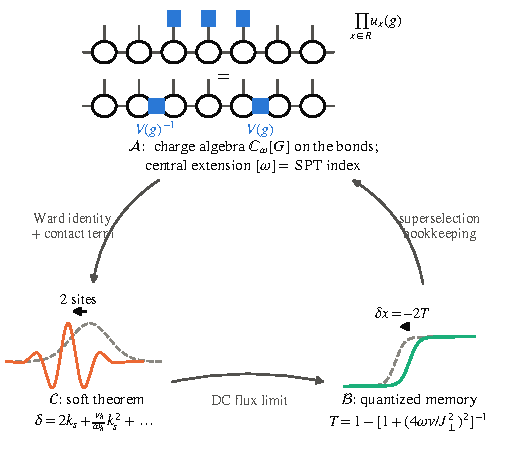
\includegraphics[width=\columnwidth]{figures/fig1.pdf}
\caption{%
The infrared triangle at finite lattice spacing. Corner $\mathcal{A}$
(asymptotic symmetry, proved): a symmetry applied to a region of a matrix
product state collapses to two bond operators $V(g)^{-1},V(g)$ at the
region's ends; on windows padded about a bond these generate the charge
algebra $\mathbb{C}_\omega[G]$, whose central extension $[\omega]$ is the
SPT index. Corner $\mathcal{C}$ (soft theorem, proved for two-body
scattering): a soft magnon of the ferromagnet exits with phase slope $2$,
i.e.\ displaced by two sites. Corner $\mathcal{B}$ (memory, proved
conditional on the scattering hypothesis H-AD): a transmitted magnon
displaces the wall by exactly $-1/s$ sites, a reflected one by zero. The
edge labels name the mechanisms; their present status is uneven and stated
honestly in the text: $\mathcal{A}\!\Rightarrow\!\mathcal{C}$ holds in the
two-body sector and is conjectural beyond it,
$\mathcal{C}\!\Rightarrow\!\mathcal{B}$ passes soft data to memory only
through the transmission probability, and
$\mathcal{B}\!\Rightarrow\!\mathcal{A}$ is charge bookkeeping within a
fixed kink sector.}
\label{fig:triangle}
\end{figure}

A dividend of the same telescoping is a lattice Noether identity: on the
vacuum, the physical charge density equals the divergence of a purely
virtual bond quantity, and for any finite-range invariant $H$ the deformed
charge $Q_k$ obeys the exact continuity equation
$[H,Q_k]=(\ec^{\ic k}-1)J_k$. One warning, learned the hard way: the
kinematic factor $\ec^{\ic k}-1$ is a property of the profile, not a soft
factor. The soft theorem has to be earned from the current.

\emph{The soft theorem.---}Fix the concrete model: the spin-$\frac12$
Heisenberg ferromagnet
$H=-J\sum_x(\mathbf{S}_x\!\cdot\!\mathbf{S}_{x+1}-\tfrac14)$. Its polarized
ground state is an exact $\chi=1$ MPS, magnons are one-particle eigenstates
with $\omega(k)=J(1-\cos k)$ and velocity $v(k)=J\sin k$, and $SU(2)$
breaks to $U(1)$, making the magnon a type-B Goldstone mode
\cite{WatanabeMurayama2012}. Write $S_{12}=\ec^{\ic\delta}$ for the exact
two-magnon amplitude, $\delta$ the continuous phase branch vanishing with
the soft momentum $k_s$, at fixed hard momentum $k_h$.

\begin{theorem}[soft magnon theorem, two-body]\label{thm:soft}
For $k_h$ in a compact subset of $(0,\pi)$ and signed $k_s\to0$,
\begin{equation}
\delta \;=\; 2\,\mathrm{sgn}(v_h-v_s)\,k_s
\;+\;\frac{|v_h|}{\omega_h}\,k_s^{2}\;+\;O(k_s^{3})
\label{eq:soft}
\end{equation}
uniformly, with $v_h=v(k_h)$, $\omega_h=\omega(k_h)$.
\end{theorem}

The zeroth order, $S_{12}\to1$, is Dyson's decoupling \cite{Dyson1956}. The
content is the next two orders. The linear coefficient is the pure number
$2$, up to the sign that records which particle is faster: independent of
the hard momentum, of the coupling, of everything. Hard data enters first
at second order, through the single even invariant $|v_h|/\omega_h$. And
the $2$ is not a scattering length---the ferromagnet's scattering length
vanishes \cite{Gongyo2016}---it is a \emph{displacement}: the soft packet
exits the collision shifted by two lattice sites
(Fig.~\ref{fig:soft-bethe}). The derivation (Appendix~B) does not solve the
model. The contact bond imposes one algebraic relation on the outgoing
amplitude; the implicit function theorem then fixes the linear coefficient
with all hard dependence cancelling. The same relation has a Ward reading:
the residue $\braket{k_h|Q_0^{\dagger}J^-_0|k_h}=2\ic\,v_h$ is charge times
velocity, the lattice image of the continuum soft-current analysis
\cite{Hamada2017,Mojahed2021}. Bethe integrability enters only as an
oracle: the closed-form expansion reproduces Eq.~\eqref{eq:soft} term by
term, and a completeness theorem for the two-magnon sector---proved by
direct diagonalization, not assumed---makes the expansion unconditional.
Exact diagonalization confirms the form factors to $2\times10^{-14}$ and
the two coefficients to $3\times10^{-10}$; real-time wavepacket collisions
reproduce the displacement reading, the coefficient $2$ to $0.2\%$.

How far beyond two bodies does this reach? Here is the strongest objection
we know, at full strength: universality \emph{fails} for unrestricted local
sources. There is an explicit four-site operator $O_\eta$ that creates the
same one-magnon state yet shifts the linear soft coefficient by
$2\ic\eta(1-\ec^{-3\ic k_h})$---a counterexample, not a technicality
(Appendix~B). What survives is a conditional statement: on the class of
Ward-covariant, no-contact sources the soft factor is universal, and we
conjecture---Conjecture~S---that for $n$-particle scattering on any
injective MPS vacuum in this class,
$M_{n+1}=2\ic k_s M_n+o(k_s)$ in wavepacket norm. The two-body case is
Theorem~\ref{thm:soft}; process independence beyond it rests on three
unproved lemmas (wave operators, uniform form-factor regularity, and the
soft-limit interchange), stated precisely in Appendix~B.

\begin{figure}[t]
\centering
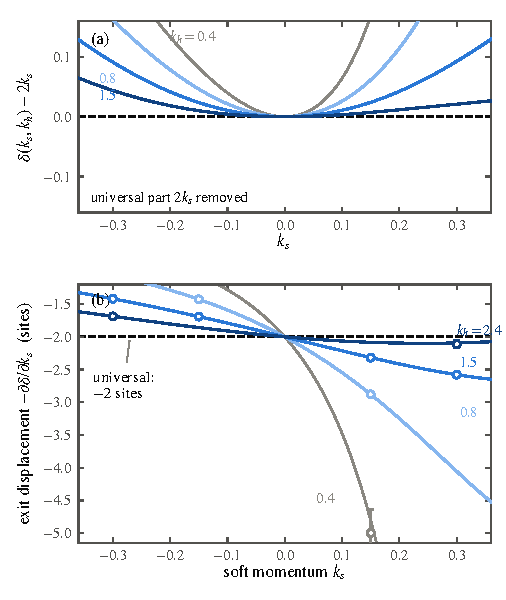
\includegraphics[width=\columnwidth]{figures/fig2.pdf}
\caption{%
The soft magnon theorem and its verification. (a)~The exact two-magnon
phase of the Heisenberg ferromagnet with its universal part removed:
$\delta(k_s,k_h)-2k_s$ vanishes quadratically for every hard momentum
$k_h$---the hard leg enters only at order $k_s^2$, with coefficient
$v_h/\omega_h$, Eq.~\eqref{eq:soft}; exact diagonalization confirms both
coefficients to $3\times10^{-10}$. (b)~The displacement reading: the soft
packet's exit displacement $-\partial\delta/\partial k_s$ for all $k_h$
(curves, exact) passes through $-2$ sites at $k_s=0$. Circles: real-time
wavepacket measurements, which reproduce the universal coefficient $2$ to
$0.2\%$. The gray curve ($k_h=0.4$) shows the non-uniformity of the
expansion as $k_h\to0$; the universal $-2$ survives it. Every soft magnon
leaves a two-site footprint, whatever magnon it scatters off---for what it
takes to drop the last qualifier, see the text.}
\label{fig:soft-bethe}
\end{figure}

\emph{Memory.---}Memory needs a wall, so change the model minimally: the
easy-axis XXZ ferromagnet, anisotropy $\Delta>1$, with two product vacua
and a domain wall between them. Send in a magnon wavepacket and ask where
the wall sits afterwards (Fig.~\ref{fig:memory}). Read the wall position
from a window $W$ around it,
$\mathfrak{X}_W=\mathrm{const}+\frac{1}{2s}\sum_{x\in W}S^z_x$. Its change
over the event is an exact operator identity, no hypotheses: the
time-integrated $U(1)$ current through the two boundary bonds of $W$, i.e.\
the zero-frequency weight of the physical boundary current. Memory is the
DC component of a current at the edge of the observation window---the
lattice image of the continuum statement that memory sits in the field at
the boundary \cite{Strominger2014,DeLuca2024}. Charge bookkeeping then
gives the memory law, in the general register.

\begin{theorem}[memory law]\label{thm:memory}
Let $G$ be compact, $\{A_\alpha\}$ a covariant family of injective MPS
vacua of any bond dimension, $H$ finite range and $G$-invariant, and fix a
kink sector between two vacua carrying charge density $\pm s$ along a
common unbroken $U(1)$. Assume the scattering hypothesis H-AD (Appendix~C):
wave operators exist for the kink-magnon event, with one reflected and one
transmitted channel of definite relative charges $\mp1$, and local decay.
Then the wall-displacement operator is
\begin{equation}
\Delta X\;=\;-\frac{1}{s}\,N_T,\qquad
\delta x\;=\;-\frac{1}{s}\braket{N_T},
\label{eq:memory}
\end{equation}
with $N_T$ the transmitted-channel projection: each transmitted magnon
displaces the wall by exactly $-1/s$ sites, each reflected one by zero, and
$\mathrm{spec}(\Delta X)\subseteq\{-1/s,0\}$ with Bernoulli variance.
\end{theorem}

The displacement is quantized by charge conservation alone: it does not
depend on momentum, anisotropy, packet shape, or any scattering phase;
those enter only through $\braket{N_T}$. The proof is bookkeeping---a
transmission changes the separated leg charge by $2$, and the wall must
absorb it at $2s$ per site---but one hypothesis is structural: the two
vacua must carry \emph{opposite} charge density along the same unbroken
direction, which forces the broken element to invert that direction, as
the spin flip does in XXZ; a bare abelian symmetry cannot produce such a
kink pair. H-AD itself we prove only for the dominant domain-wall sector
of the XXZ chain, conditional on an explicitly stated sector-reduction
hypothesis; for the full chain it remains an assumption (Appendix~C).
Sparse-sector numerics on chains of $160$ sites confirm
$\delta x=-2\braket{N_T}$ at $s=\frac12$ to $0.004$ sites.

In the reduced sector the kink-magnon problem is a side-coupled (Fano)
level, giving the closed form
$t(k)=[1+\ic J^{2}/4\omega(k)v(k)]^{-1}$ with $\omega(k)=J(\Delta-\cos k)$;
the measured reflection matches this over $\Delta\in[1.5,12]$ to
$0.9$--$5.8\%$ with no fitted parameter (criterion $8\%$, fixed in
advance). As $k\to0$,
\begin{equation}
T(k)=16(\Delta-1)^{2}k^{2}+O(k^{4}),
\label{eq:softzero}
\end{equation}
so a soft magnon is totally reflected and leaves no memory: the memory
effect has an Adler zero of its own. Whether the zero's coefficient is
universal---a function of the kink's asymptotic data alone---we have not
established; that remains a conjecture.

Now the refutation. The continuum triangle suggests a dictionary: memory
$=$ DC limit of the soft factor, summed over the event. That statement is
\emph{false} in the XXZ chain, twice over: the displacement per
transmission is fixed by charge conservation whatever the scattering phase
does, and a purely transmitting wall with identically zero phase shift
still displaces by exactly $-1/s$. The soft factor is a
phase; the memory quantum is a charge. What survives---and is proved---is
the pair above: memory is the DC weight of the boundary current, and soft
data reaches it only through the transmission probability. We regard this
not as a failure of the triangle but as its lattice sharpening: the third
corner closes through charge transport, not phase accumulation.

The remaining edge closes at the level of bookkeeping, and only there:
under finite-range dynamics the vacuum-pair label of the kink sector is
rigid at finite times, and the displacement obeys
$2s\,\delta x+(q_{\rm out}-q_{\rm in})=0$ within that fixed sector. That
the memory \emph{reconstructs} the asymptotic transformation which acted
remains open.

\begin{figure}[t]
\centering
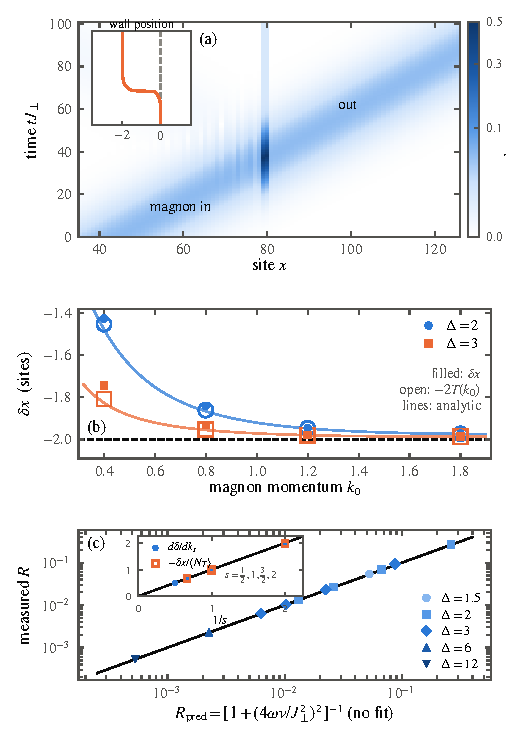
\includegraphics[width=\columnwidth]{figures/fig3.pdf}
\caption{%
The quantized memory effect in the XXZ chain ($\Delta>1$).
(a)~Space--time record of one event ($\Delta=3$, $k_0=1.2$, $N=160$):
flipped-spin density as a magnon wavepacket crosses the wall. Inset: the
wall position, which steps back by two sites during the collision and stays
there---the permanent record. Across the scan the displacement obeys
$\delta x=-2\braket{N_T}$ to $0.004$ sites. (b)~Displacement versus
momentum: filled symbols $\delta x$, open symbols $-2$ times the measured
transmission, curves the parameter-free Fano prediction. (c)~The measured reflection collapses onto
$R=[1+(4\omega v/J^{2})^{2}]^{-1}$ across $\Delta\in[1.5,12]$,
$k_0\in[0.4,1.8]$, to $0.9$--$5.8\%$; as $k_0\to0$ transmission vanishes
quadratically, Eq.~\eqref{eq:softzero}: a soft magnon leaves no memory.
Inset: the spin-$s$ falsifier of Conjecture~B. Soft phase slope (filled,
rings up to $480$ sites) and memory quantum $-\delta x/\braket{N_T}$
(open, wavepacket runs) against the single line $1/s$, for
$s=\frac12,1,\frac32,2$ (memory: $s\le\frac32$). Both follow the charge
datum, not the constant $2$.}
\label{fig:memory}
\end{figure}

\emph{One invariant, read out twice.---}Two $2$'s appear above: the soft
phase slope of Theorem~\ref{thm:soft} and the spin-$\frac12$ memory quantum
$1/s$ of Theorem~\ref{thm:memory}. We conjecture---Conjecture~B---that both
equal $|q_{\rm hard}|/s$, the hard particle's $U(1)$ charge in units of
the vacuum spin density: one asymptotic-charge datum read out as a phase
in corner $\mathcal{C}$ and as a displacement in corner $\mathcal{B}$.
The conjecture was built to fail at $s\neq\frac12$, where the candidate
laws $1/s$ and the constant $2$ separate; it survived
(Fig.~\ref{fig:memory}c, inset). Two independent implementations measured
the phase slope $=1/s$ across $s\in\{\frac12,1,\frac32,2\}$ and the memory
quantum $=-1/s$ across $s\in\{\frac12,1,\frac32\}$, within pre-registered
$8\%$ bands (measured deviations $\le1\%$ at clean kinematics); an exact
two-magnon contact computation gives the slope $1/s$ in closed form, with
all hard dependence cancelling. The $|q_{\rm hard}|$ factor is untested:
every leg so far carries $|q|=1$, and a charge-$2$ bound-state projectile
is the next falsifier.

\emph{Where the SPT index lives.---}Corner $\mathcal{A}$ made $[\omega]$
the central extension of the soft charge algebra; does it show up in soft
amplitudes? The answer is a rigidity dichotomy, and it is proved
(Appendix~D). In the \emph{bulk}, a closed symmetry insertion has two
endpoints whose projective multipliers cancel exactly, and every normalized
soft coefficient is a continuous function along symmetric gapped
deformation paths: nothing bulk is a topological invariant without a
separate local-constancy proof. Along a symmetric path through the AKLT
phase, a natural bulk soft-charge coefficient moves from $0.125$ to
$0.240$ with the SPT class fixed.
At an \emph{unpaired endpoint} the situation inverts: the compensated soft
residue is an operator on the $\chi$-dimensional edge register whose
centered charge has spectrum in the $[\omega]$-shifted lattice
$q^\circ_\omega+\mathbb{Z}$ and dimension at least that of the smallest
$\omega$-projective representation. For the AKLT half-chain the residue is
exactly $-\frac{1}{2}[1-(2b^2-1)^L]\,Z\to-Z/2$ along the entire path:
eigenvalues $\pm\frac12$, rigid, while the bulk coefficient drifts. The
topological data of soft physics concentrates at the boundary. Physical
edge statements carry the hypothesis H-split above, and charge bookkeeping
then quantizes edge-memory outcomes exactly as in Theorem~\ref{thm:memory}:
what is protected is the memory's \emph{capacity}---a projective multiplet
no symmetric perturbation can split---not any particular amplitude. That an AKLT boundary magnon
actually writes to it, we state as a conjecture with a definite
Hamiltonian and a pre-registered test (Appendix~D).

\emph{Outlook.---}The topological data of the chain thus concentrates in
a boundary soft algebra, $\mathbb{C}_\omega[G]$ at the ends, in structural
parallel to the celestial program's discovery of symmetry towers at the
boundary of spacetime \cite{Strominger2017}. The symplectic origin of this
charge algebra---the moment-map geometry of the MPS manifold behind the
bond operators---is deferred to forthcoming work. The asymmetry of our
opening has meanwhile dissolved: the wall is a broken asymptotic symmetry
made visible, and the magnon's soft phase and the wall's memory measure
one conserved charge crossing an observer. The infrared structure of gauge
theory and gravity, long tied to null infinity, fits on a chain of spins,
where every step of it can be checked.

\begin{acknowledgments}
We thank D.~Giulini for discussions. % CONFIRM WITH TJO before submission
\end{acknowledgments}

\appendix

\section{Corner A: the asymptotic charge algebra}\label{app:cornerA}

Ground truth: repository shards \texttt{theory/corner-a.md},
\texttt{corner-a-kinks.md}, \texttt{corner-a-goldstone.md} (claim rows WI,
A1, A2, G0, all PROVED through the adversarial verification loop recorded
there); numerical certificates in Appendix~E. Throughout, $\alpha$ labels
vacua, $H_\alpha=\{g:g\cdot\alpha=\alpha\}$ the unbroken subgroup, and
phases are normal-ordered so that the extensive phase of the truncated
symmetry is removed.

\emph{Truncated symmetry (WI).} For a finite region $R=[a,b]$ and any
$g\in G$, exactly and with no limit,
$U_R(g)\ket{\psi(A_\alpha)}=\ec^{\ic|R|\theta_\alpha(g)}
\ket{\psi(T^{(g)}_R)}$, where $T^{(g)}_R$ carries $A_\alpha$ outside $R$,
$A_{g\cdot\alpha}$ inside, and two bond insertions: $V_\alpha(g)^{-1}$ on
$\partial_-R$ and $V_\alpha(g)$ on $\partial_+R$. The window must contain
one site beyond each cut (or carry explicit edge-bond insertions); with
interior bonds only, the identity is false, and the orientation of the two
insertions matters---both failure modes are exhibited numerically in the
certificate.

\emph{Unbroken case (A1).} (a)~Half-infinite strings act on states exactly
as single bond insertions, and the convergence is eventually constant on
every local algebra, not asymptotic. (b)~They are implemented by a strongly
convergent operator sequence if and only if $V_\alpha(g)$ is scalar.
(c)~Two insertions give the same state iff they differ by a scalar, so the
endpoint states form a $PGL(\chi)$-torsor. (d)~On windows padded about the
bond the map $M\mapsto$ insertion is injective, and the insertions realize
a linear representation of the twisted group algebra
$\mathbb{C}_{\omega_\alpha}[G]$ in which the multiplier acts nontrivially;
padding is necessary---an explicit $\mathbb{Z}_2$-symmetric counterexample
shows the unpadded action is ill defined. On states the multiplier dies and
what remains is a homomorphism $G\to PGL(\chi)$; what $[\omega_\alpha]$
obstructs is lifting it to an honest unitary representation.
(e)~\emph{Open (H-split):} that these endpoint states are normal states of
the physical half-infinite algebra---equivalently that
$\mathbb{C}_\omega[G]$ acts on a physical edge Hilbert space---is not
proved; the expected route is the split property. Every physical-edge
statement in this Letter carries this hypothesis explicitly.

\emph{Broken case (A2).} For $g\notin H_\alpha$, every finite truncation
stays in the vacuum sector (a kink-antikink pair at the two ends); the
half-infinite limit exists in the weak-$*$ sense only, with an exponential
rate, and lands in the kink sector $\mathcal{K}_{\alpha,g\cdot\alpha}$,
disjoint from the vacuum folium. The jump is invisible at every finite
truncation and created entirely by the surviving end. Under the
transitivity hypothesis (T), vacuum pairs form
$(G/H_\alpha)\times(G/H_\alpha)$ and the complete diagonal invariant is the
double coset in $H_\alpha\backslash G/H_\alpha$; for $G=SU(2)$ broken to
$U(1)$ this is the relative angle of the two vacuum axes. Without (T) the
classification holds per orbit. Two load-bearing gaps are recorded in the
shards and respected here: H-split above, and the absence of a
$g$-uniform statement when the vacuum manifold is continuous.

\emph{Currents (G0).} For any generator $\xi$ and finite-range invariant
$H$: $[H,q_x(\xi)]=j_{x-1|x}(\xi)-j_{x|x+1}(\xi)$ with the local cut
current, and in wavepacket form $[H,Q_k]=(\ec^{\ic k}-1)J_k$. On the
vacuum, the charge density acts as the lattice divergence of a virtual bond
quantity---the potential is the fundamental object, as a theorem. The
finite-window Fourier identity carries two $\Theta(1)$ boundary terms; the
clean $(1-\ec^{\ic k})$ form holds only in the stated $\delta$-normalized
sense. The kinematic factor supplies no soft theorem (a withdrawn overclaim
is recorded as a refuted row in the claims ledger).

\section{Corner C: the two-body soft theorem and its limits}
\label{app:soft}

Ground truth: \texttt{theory/soft-current-recon.md} (row S2-2body, PROVED),
\texttt{theory/oracle-bethe.md} (oracle facts O1--O10, verification role
only), \texttt{theory/ml2-completeness.md} (row ML2, PROVED),
\texttt{theory/ml4-ward-reduction.md} and
\texttt{theory/ml5-universality.md} (rows ML4-A, ML4-Ward, ML5-A/B PROVED
as conditional implications; ML5 unrestricted REFUTED).

\emph{Derivation of Theorem~\ref{thm:soft}.} The exact current of the
model is $j^-_{x,x+1}=\frac{J}{2}(S^-_{x+1}-S^-_x)P_{x,x+1}$. A two-magnon
eigenwave is free away from contact; writing the incoming coefficient as
$1$ and the outgoing as $s(k_s,k_h)$, the single contact bond imposes
\begin{equation}
(2z_h-z_sz_h-1)\,s+(2z_s-z_sz_h-1)=0,\qquad z=\ec^{\ic k},
\label{eq:contact}
\end{equation}
whose unique analytic solution near $k_s=0$ has $k_s$-coefficient $2\ic$,
all hard dependence cancelling; the continuous logarithm gives
Eq.~\eqref{eq:soft}, with remainder uniform on compact hard sets. The Ward
reading: the state $Q_0\ket{k_h}$ is the Bethe descendant with one rapidity
at infinity, and
$\braket{k_h|Q_0^\dagger J^-_0|k_h}=2\ic v_h$; dividing a hard external-leg
reduction by the energy shift $v_h k_s$ cancels the velocity and leaves the
$2$. Symmetry alone does not prove the theorem: the current has an
orthogonal contact component, and what makes it subleading in the two-body
sector is energy-shell matching plus $C^1$ regularity of the on-shell
trace (an abstract cancellation lemma proved in the shard), not the Ward
identity. Completeness of the two-magnon resolution---scattering states,
one bound band, descendants, and one singular vector on even rings---is
proved by direct Jacobi diagonalization; no Bethe completeness is assumed,
and integrability appears nowhere in the hypotheses.

\emph{The universality boundary.} With the four-site local operator
$D=S^-_0S^-_1-S^-_1S^-_2+S^-_2S^-_3-S^-_0S^-_3$, the source
$O_\eta=S^-_0+\eta D$ creates the same one-magnon amplitude as $S^-_0$ but
shifts the linear soft coefficient of the induced two-body amplitude by
$2\ic\eta(1-\ec^{-3\ic k_h})$. Unrestricted process independence is
therefore refuted. The repaired statement (proved as a conditional
implication) holds on the source class $\mathcal{S}_W$ defined by five
conditions---vanishing soft intercept and first contact jet, second-derivative
norm control, an exhaustive LSZ decomposition, and reduced-channel
matching---and Conjecture~S asserts universality on exactly this class.
Open, and stated as such: infinite-volume wave operators (ML1), uniform
form-factor regularity including the $k=\Theta(1/N)$ regime (ML3), the
$n\ge2$-hard channel (ML4 beyond one hard leg; the fixed-volume formulas
are an off-shell interpolation whose naive volume-uniform reading is
refuted), microscopic membership in $\mathcal{S}_W$, and the limit-order
control (ML6).

\emph{Spin-$s$ slope.} For the spin-$s$ ferromagnet the same contact
algebra (non-symmetrized free extension plus a double-occupancy channel)
gives the closed-form two-magnon amplitude with soft phase slope $1/s$,
hard dependence again cancelling; two independent derivations agree to
$10^{-15}$. This exact computation is the analytic half of the
Conjecture~B falsifier; it has not yet passed through the verification
loop and is counted as evidence, not theorem.

\section{Corner B: flux identity, memory law, Fano reduction}
\label{app:memory}

Ground truth: \texttt{theory/memory-quantization.md} (rows M-flux PROVED;
M-quant PROVED conditional on the hypothesis D18 $=$ H-AD; Mq-AD3 PROVED
conditional on the sector-reduction hypothesis Mq-E),
\texttt{theory/memory-quantization-general.md} (row M-quant-G, PROVED as a
conditional implication), \texttt{theory/corner-b-draft.md} (rows K1--K3,
B3 PROVED; K4 CONJECTURE; row M REFUTED).

\emph{Flux identity (exact).} For any state, any window $W=[a,b]$, and any
finite times, $\frac{d}{dt}\mathfrak{X}_W$ equals $\frac{1}{2s}$ times the
difference of the two boundary-bond currents; integrating,
$\delta x=\frac{1}{2s}[\tilde{\jmath}_{a-1|a}(0)-\tilde{\jmath}_{b|b+1}(0)]$,
the zero-frequency weight of the physical boundary current. No kink,
spectral, or asymptotic hypothesis enters. (An earlier reading of this
identity through virtual bond data was deleted during verification; the
current here is physical.)

\emph{Hypothesis H-AD.} Wave operators $W_\pm$ exist for the selected
kink-magnon vector and are complete on its sector; the outgoing space
splits into reflected and transmitted channels with definite relative
charges $q_{\rm in}=q_L=-1$, $q_T=+1$; local observables decay on the
moving legs; and limits are taken in the stated order (infinite volume,
then time, then window). For Theorem~\ref{thm:memory} in the general
register these charges, the density jump $2s$, and summable charge
deviations from the two vacua (an $\ell^1$ kink class) are the only inputs:
conservation of the regularized charge $2s(\mathfrak{X}_W-c)$ plus leg
bookkeeping gives $2s\,\delta x+(q_{\rm out}-q_{\rm in})=0$ per channel,
hence Eq.~\eqref{eq:memory}; the quantum for a charge-$\nu$ transfer is
$-\nu/2s$. The structural remark in the text is the shard's: covariance forces
$\omega_{g\cdot\alpha}(\xi)=\omega_\alpha(\mathrm{Ad}_{g^{-1}}\xi)$, so if
the broken element commutes with the unbroken direction
($\mathrm{Ad}_{g^{-1}}\xi=\xi$, as for any abelian $G$) the two vacua carry
\emph{equal} densities and no such kink pair exists; the required inversion
is supplied by a Weyl-type element, as the spin flip in XXZ. Nothing in compactness, injectivity, or finite range implies
H-AD itself; it is proved here only where stated next.

\emph{Sector reduction and the Fano level.} In the XXZ chain at $s=\frac12$
the incoming component with at most three domain walls, under the
enumeration hypothesis Mq-E (verified explicitly at $N=14$; all-volume form
open), is unitarily a two-sided tight-binding chain with one side-coupled
level---the flat kink state, whose bondwise annihilation by the exact kink
Hamiltonian is proved. Kato--Rosenblum and a Feshbach analysis then give
H-AD for this reduced dynamics: trace-class perturbation, complete wave
operators, no singular-continuous spectrum. Eliminating the side level
yields $t(k)=[1+\ic J^2/4\omega v]^{-1}$ and Eq.~\eqref{eq:softzero}.
Leakage of the full chain out of the reduced sector is measured at
$O(\Delta^{-2})$ (probabilities $0.10/0.03/0.008$ at $\Delta=2/4/8$); it
affects $T(k)$, not the conservation laws. Full-chain H-AD and the
universality of the soft-zero coefficient remain open and are tracked as
such in the claims ledger.

\emph{Refutation of the naive dictionary.} The brief's Conjecture~M
(``$\delta x$ is the DC limit of the soft factor'') fails on two counts:
the channel quantum is independent of the scattering phase once the
channels exist, and a phaseless purely transmitting wall still displaces
maximally. The refuted row is retained in the ledger with its
counterexamples; the surviving pair is the flux identity plus
Eq.~\eqref{eq:memory}.

\emph{Label rigidity.} Under stationary vacua and finite-range
(Lieb--Robinson) dynamics the factorized vacuum-pair boundary label of the
kink sector is preserved at all finite times, so $\delta x$ is motion
within a fixed sector, not a change of sector. The thermodynamic
uniqueness/flatness of the kink family (a $\mathbb{Z}$-torsor reading)
remains a conjecture with finite-volume evidence.

\section{The SPT rigidity dichotomy}\label{app:spt}

Ground truth: \texttt{theory/spt-rebuild.md} (rows SPT-B-mult, SPT-B$'$,
SPT-E-AKLT, SPT-E$'$, SPT-T$'$, SPT-D$'$, SPT-M$'$ all PROVED with the
hypotheses below explicit; SPT-M$'$-dyn CONJECTURE; the earlier pointwise
bulk-blindness claim and the all-orders edge no-go both REFUTED and
retained as negative rows).

\emph{Bulk (deformable).} A closed on-site insertion leaves
$V(g)\otimes\bar V(g)$: the multipliers cancel exactly, for every lift, so
no closed-bulk amplitude carries a projective anomaly. This does not make
bulk data blind to the phase---adjoint representation content
distinguishes Pauli-projective from scalar conjugation---but it is
deformable: along any common-gap symmetric path with continuous external
data, every normalized bulk coefficient is continuous. On the anisotropic
AKLT family ($A^x_b\!\propto\!X$, $A^y_b\!\propto\!Y$, $A^z_b\!\propto\!Z$)
the soft-charge coefficient is $C_{\rm bulk}(b)=b^2/4(1-b^2)$:
$\tfrac18$ at the AKLT point, $0.2402$ at $b=0.7$, same phase, same
$[\omega]$.

\emph{Edge (rigid).} On the fixed $\chi$-dimensional Schmidt register of a
half-chain, the compensated endpoint residue of a symmetry string is
$V(g)$ itself, and the Hermitian charge residue is the centered generator
$Q_{\rm edge}=-\ic X^\circ$, lift-gauge invariant, with spectrum in the
shifted lattice $q^\circ_\omega+\mathbb{Z}$ and every irreducible summand
of dimension $\ge d_\omega$ (the minimal $\omega$-projective dimension;
$>1$ whenever $[\omega]\neq0$). For the AKLT family the finite-window
residue is exactly $-\frac12[1-(2b^2-1)^L]Z$, with limit $-Z/2$
independent of $b$; the trivial comparison tensor gives $0$. The
half/integer offset is pinned by the global group ($O(2)$ here, or the
$SU(2)$ cover); a bare $U(1)$ does not protect it.

\emph{Edge memory.} Given H-split, an edge-resolved H-AD, charge
conservation, and definite channel charges,
$\Delta Q_{\rm edge}=-(Q_{\rm bulk,out}-Q_{\rm bulk,in})$, with channel
outcomes in $\mathbb{Z}$ (for the AKLT doublet, in $\{-1,0,1\}$)---the
same bookkeeping as Theorem~\ref{thm:memory} with edge charge in place of
wall position. Protection is capacity protection: the projective multiplet
cannot be split symmetrically. That the specific open AKLT parent
Hamiltonian with boundary coupling $P^{(S=2)}_{0,1}$ has a nonzero
edge-changing reflection amplitude on an open momentum interval is
conjecture SPT-M$'$-dyn; the deciding half-chain scattering computation,
with pre-registered acceptance gates, is specified in the shard. A null
result there refutes that conjecture only, not the registered endpoint
theorems.

\section{Numerical certificates}\label{app:numerics}

Every theorem above carries an independent machine-checked certificate
under \texttt{theory/checks/} (nine checkers, all passing, each with
documented failing ``red'' mutations), and the quantitative claims of the
text trace to committed data files: exact-diagonalization form-factor
residuals $\le1.6\times10^{-14}$ and coefficient fits to
$2.2\times10^{-10}$ (\texttt{soft\_current\_recon\_check.py}); two-magnon
completeness on rings up to $26$ sites
(\texttt{ml2\_completeness\_check.py}); the flux identity to
$3.4\times10^{-16}$ (\texttt{mquant\_check.py}); the wavepacket memory scan
(\texttt{memory-scan-1.json}: $N=160$, sparse kink-sector propagation,
trapped weight $<10^{-6}$, $|\delta x+2\langle N_T\rangle|\le0.004$ sites);
the Fano cross-check ($0.9$--$5.8\%$ over
$\Delta\in\{1.5,2,3,6,12\}$, pre-registered $8\%$ criterion); the spin-$s$
falsifier and its independent cross-check
(\texttt{spin1-bc-falsifier.json}, \texttt{spin1-bc-crosscheck.json}:
ansatz-free ring spectra to $N=480$ plus real-time collisions, slope
deviations from $1/s$ below $0.5\%$ extrapolated; wavepacket memory ratios
within $1\%$ at clean kinematics); and the SPT deciding computation
(\texttt{spt\_rebuild\_check.py}: bulk coefficient and edge residue to
stated tolerances, sign and phase-gauge mutants failing). Figures 1--3 are
generated from these committed files by
\texttt{paper/figures/make\_figures.py}; no number is hand-entered.

\bibliography{refs}

\end{document}
